

\documentclass[notitlepage]{report}
\usepackage[left=1in, right=1in, top=1in, bottom=1in]{geometry}
\usepackage{graphicx}
\usepackage{titling}
\usepackage{lipsum}
\usepackage{amsmath}


\pretitle{\begin{center}\Huge\bfseries}
\posttitle{\par\end{center}\vskip 0.5em}
\preauthor{\begin{center}\Large\ttfamily}
\postauthor{\end{center}}
\predate{\par\large\centering}
\postdate{\par}

\title{On the possibility of probing deep-quantum mechanics}
\author{An investigation into theoretical foundations for physics}
\date{\today}
\begin{document}

\maketitle
\thispagestyle{empty}

\begin{abstract}
The Xyston project is a bold attempt at probing a possible deeper reality than quantum mechanics, called deep quantum mechanics. In this paper, the motivation for that project is outlined, a philsophical foundation is chosen and the reasoning behind the choice of philosophical foundation. 
\end{abstract}



\section*{The quest for intuitive understanding of physics}
Since the birth of quantum mechanics, the science of physics has developed into the Standard Model of particle physics, a hybrid between Quantum Physics and General Relativtity. The two theories are operating at different scales, with an unclear boundary and starkly different mathematical foundations. This uneasy coexistence is bridged by a collection of tools such as quantum renormalization, providing a techniques to adjust the quantum formalism to the desired scale. At higher scales, quantum effects even out so that classical mechanics (the laws of Newton) can be used, and at even higher scales - theory of general relativity. Although tremendously successful, there are many crucial parts of the framework that simply work, when given the right parameters, that produce excellent predictions, but without giving an intuitive way to make sense of why it works, or why the parameters are just the way they are. The theories are lacking a proper intuitive foundation.

An example of this in the macroscopic scale, is that the Standard Model contains many parameters that are put in there, in order to make the model work. In order to explain these parameters, theories have been created with the explicit goal of understanding the parameters in more detail. The expansion of the universe for example,  was not included in the model after being proven to exist, but rather as an explanation for a parameter the model needed. As for the expansion of the universe, more and more evidence accumulate supporting this idea. But there is no way to estimate the strength of the expansion outside the standard model. It remains a fact that the strength of the universal expansion - the hubble constsant - is defined in terms of making the model work, leaving no room for alternative theories. Currently, with other evidence in support of the universal expansion, the Hubble constant is a parameter drawn from a viable theory that is likely to be correct. But even so, it is also, undeniably, an error term in the equation, estimated as the catch-all explanation for all remaining redshift, unexplained by other means.  This circular double role, of being both defined in terms of set parameter, and then in the next instance used to define the parameter leaves no room for other redshift inducing mechanisms yet to be discovered, without also reducing the Hubble constant. This is an often overlooked weakness in the Standard Model, and pointing this out can be seen as critique of the Standard Model itself. But in reality, it is only an critique of the explanatory power, not the predictive power of the theory.

There is a similarity in Quantum Mechanics. The quantized nature of phenomena on the quantum scale, the counter-intuitive phenomena like entanglement are studied in terms of their abstract math, and not in terms of an intuitive model. Students are taught to "get used to it" , and focus on the predictive power of the model.  It is possible that its undeniable success and predictive power might have become an obstacle to a deeper understanding, or even probing into a possible deeper layer than the quantum world itself. Here too, the theory lacks an intuitive foundation.

However, not all scientists see this as  problem. Some would argue that it is not necessarily the case that reality works in a way that is intuitive, that is well matched to the way humans process information. There might be hard limits to our understanding. Reality doesn't have to respect those limits. If this is true, the right way to deal with this constraint on our imagination is to work through it, learn the maths, get used to its quirks and peculiarities, and not waste time insisting that a better, more intuitive explanation and formulation of quantum mechanics exists. This is not a bad argument. 

Others remain convinced that the standard QM conceptualization of the quantum world is less than it could be, that a new representation would make it more intuitive. This increase in intuitive comprehension could propel our understanding to new heights, bolster our capacity to formulate questions, open new doors to deeper questions about the nature of reality, whilst retaining  prediction power. Both sides of the argument have valid points, but I confess to joining the second camp. When asked to  relinquish the possibility of being able to intuitively understand, I have no choice but to answer: No! This I cannot do. (It feels as if my world depends on it.)

To those in this second camp - my camp - it's a widespread intuition that the main fault line of our current understanding, represented by the Standard Model of particle physics, is the blurry transition from a quantized theory to a continuous one. If this intuition is correct, it is possible that a choice must be made whether to view reality as  fundamentally quantized, or as fundamentally continuous. This is not so easy as separating Quantized Quantum Mechanics from continuous General Relativity. Key parts of Quantum Mechanics like the Schrödinger wave equation remain formulated as a continuous function. Because Quantum Mechanics is both quantized and continous, choosing a preferred frame has profound implications.


\section*{What is a good foundation?}
The current foundation of modern physics is Quantum Mechanics,  adapted from Maxwells equations and developed into a powerful framework now over 100 years old. To avoid wasting time in the wilderness of fancyful ideas, we must seek a foundation, quickly build a physics of some sort on top of it, and then immediately try to make falsifiable predictions that can help us make contact with existing theories. When seeking a new foundation for physics, there are not much to guide us. Luckily, 100 years of experience has provided clues as to what a new theory must contain to be what we seek.  In the paper Quo Vadis Quantum Mechanics  \cite{QuoVadis1ACElitzur}, A. C. Elitzur summarizes what we yearn for in a new theory:

\begin{enumerate}
	\item  Beauty and elegance: The feeling of understanding how something complex can arise from something simpler.
		\item  Continuity : Builds or meshes beautifully with current theories, showing they are special cases in a broader more general theory.
	\item  Unity : Explaining several things we don't understand through a single underlying mechanism
	\item  Sacrifice : Long held truths must be reconsidered, perhaps by their proofs being seen in a new light.
	\item Novel predictions : Surprising new predictions.
	\item Unepected dividends : A new theory provide a new angle to understand other problems in different domains.
\end{enumerate}

Only the first two, Beauty and Continuity can inform our choice of foundation, because the other four simply are characteristic of a successful theory. As for beauty - simplicity and elegance are related terms. A commitment to Beauty requires us to formulate as minimal starting point as possible, and then stick to it and see where it leads. If we choose the wrong foundation, our efforts are doomed to fail, and the theory will end in bad predictions about reality, self inconsistency or both. This is not as bad as it sounds, because even if the project fails, something can be learned from a structured and careful inquiry into any foundation. If we, on the other hand and against all odds, choose the correct foundation, the theory is bound to bloom, to unfold into a theory that explains all the other theories we have developed with perfect clarity. Herein lies the boldness of the undertaking. A commitment to Continuity requires us to pay sufficient respect for the power and usefulness of existing theories, and seek to explain them in a new way rather than attempt to disprove them. Until we can make testable predictions, a new theory is merely a philosophical argument ornamented with maths. 

This brings me to an important point: We shouldn't have unreasonable expectations. There might well be a period of time in the development of a new foundation, where the commitment to beauty and the commitment to continuity come into conflict. There might be a developmental stage where the commitment to beauty must take precedence to conformance with existing theories that we know to have great prediction power. In this phase, a new theory must target the other characteristics of a good theory, provide surprising new predictions and insights, anchored in the foundation assumptions of the theory. It is crucial to remain true to it's foundation.

\section*{The act of quantization }
A committment to Beauty also means studying the parts of our theory where we feel least at easy. As previously mentioned the transition from quantized to continous is proving a challenge to the intuition. For this reason, this is where I will start.

In 1908, Max Planck was able to solve the problem in black body radiation known as the ultraviolet catastrophe. He did this by applying quantization, that is taking an continuous mathematical function, assuming it is not infinitesimally divisible, but that there is a smallest possible subdivision, resulting in a range of minimal units, such as Planck Length, Planck Time Planck charge etc. Let us consider quantization as a tool in the toolbox of the physicist, that can be used to change the dynamics of a model. If such a quantized model conforms to experimental data, this suggest that the system is quantized, and that we use a quantized model to make predictions about this system. Otherwise, we assume continuity and prefer the simpler and more beautiful continuous models. However, it remains self evident that out of all quantized systems, a subset exists that has sufficient resolution that the "steps", "pixels"or "increments" become so small they they cannot be individually detected. If such a system also behaves in a predictable way, it might be accurately approximated by a continuous model. In fact, a continuous definition is favoured because of the elegance and beauty of analytical formulations.

Quantum theories are obviously quantized, but this does not go as deep as it first may appear. They are all quasi-linear, only partially quantized algebras of states and their evolution. It could be argued that Quantum theories are minimally quantized - quantized only insofar of applying quantization produces better results. This is logical, given that Quantum Mechanics branched off from classical physics, particularly the study of electromagnetic fields through Maxwells equations. 
But this means that inQuantum Mechanics, two distinct styles of thinking are in play at the same time. Both quantized and continuous approaches are combined with sometimes great beatuy and other times uneasy co-existence. General relativity on the other hand, is a completely continuous formulation of the relationships between mass, energy and time one the macroscopic scale, without any quantized components at all. What should we make of this?
All we know is that the problem of Black Body radiation could not be solved in a continuous frame of reference, and required the introduction of quantized values, and from came much more than just a solution to a pesky little problem, it yielded a completely new theory, a new beginning for physics. It seems to me that the history of Quantum Mechanics is trying to tell us one thing - there is something special about the act of quantization, and it might be worthwhile to consider the philosophical implications of having access to this tool at all. To explore this, we begin by asking a simple question: Where does the quantized end and the continous begin?

\section*{Inverse quantization}
As soon as we have invoked the idea of $quantization$, we have also invoked it's opposite, $continuization$. For the duality to be completed, this too must be described. But what emerges from the $continuization$ of a quantized system? one possible result is to generate intermediate states, between the quantized one that does not exist in the quantized system. However, if we do not allow for such intermediate states, the ratios and relationships that are expressed in the continous equations take on a new value - that of probabilities. For example, if two perpendicular states are 50\% likely to happen, then the average angle realized will be 45 degrees. 

This corresponds to $\frac{cos(\theta) + sin(\theta}{2}$.


The relationship between quantum mechanics and general relativity is that of emergent continuous behaviour from a quantized subsystem. The stone in an asteroid orbiting a planet might have quantum states, but as the scale is increased, the quantized states even out and produce average behavior. If there is a systematic nature to the quantized output, an approximation is possible, and this can often be represented analytically by a mathematical relation, specified by a mathematical function. If the underlying resolution of the quantized scale is high enough, there is no way to discern an objective continuous reality from a continuous approximation to a sufficiently high resolution quantized reality. The discerning factor becomes the usefulness of the equation. This could lead us, all other things being equal, to assume a continuous nature of a quantized reality. Given sufficiently high resolution, we can argue that a quantized system can only be effectively understood through a continuous approximation. Any stochastic system, even a quantized one exhibit the emergence of continuous mathematical relationships. For quantum mechanics, this is seen through the continuous nature of quantum probabilistic, the wave function etc. Quantum mechanics is in fact mostly about probabilities, and therefore it is mostly continous. Continuization of a quantized system can take many forms, and probabilistic is the first stage of continuization.

\section*{Emergent quantization from continuous systems}
Our next question comes naturally. Is this a one way street, from quantized to continuous? Or can quantization also emerge spontaneously out of  a continuous system? The short answer is yes. Consider any quantized system and ask, where does the quantization actually come from? The answer can only be one of two options. It is either fundamental, an aspect of objective, final, or root-reality  - or the quantization is scale dependent, i.e an emergent property of a deeper level of reality. This deeper level can itself be either quantized or continuous. 
We can know this because it is possible to imagine a continuous system interacting in such a way, that it produces quantized states. If you look carefully, you might be able to spot it in nature. A small stream of water on inclined tarmac might form wavefronts at specific intervals, the intervals becoming shorter as the amount of water increases but the height of the wavefront remains constant. The phenomena is known as roll-waves, and is the result of the surface tension of water and the friction of the tarmac interacting in such a way that wavefronts occur. 
Imagine then a scenario, where your instrumentation were only able to measure if a wave passed, or not. All you would see was binary information about wave or not wave. After studying such roll waves and seeing only binary information about their existence, might one  not reasonably conclude that water running down a tarmac slope travels in quanta, in discrete packets of water? Seeing this natural phenomena, we can at once confirm that quantized phenomena might arise from continuous processes. 

But notice how this only pushes the problem into a smaller scale level. The quantized nature of roll waves might emerge from a continuous process, but this continuous process might in turn be emergent from a much finer quantized process - in this case, on the subatomic quantum scale. This observation is important, because even if we take the assumption that everything is quantized, we cannot firmly close the door to the possibility that the quantization we observe is the result of emergent quantization at a deeper level, even a continous one.
Quantum Mechanics is a case in point. We know that Quantum systems exhibit quantized states, called eigenstates, but we cannot know that these eigenstates are fundamental. Quantum Darwinisim is a theoretical framework that attempts to create a framework for understanding a possible sub-quantum mechanics. Quantum Darwinism attempts to use evolution and competition between forces,resulting in stable equilibria, to explain the stable pointing states exhibited by quantum systems. 

Stable equilllibria is studied in many fields including demography, economics and meteorology, and are caused by counterbalancing forces that oscillate back and forth until they reach remarkably stable balancing points over time. Given a finer subdivision than the quantum scale, we can imagine many different mechanisms that would produce stable equilibria, and all we have to do is to associate them with the quantized eigenstates of quantum mechanics to have a rough but intuitive model of sub-quantum mechanics.
Far from proving it, but Quantum Darwinism has been able to create an intuitive argument about the existence of a sub-quantum mechanics that cannot be easily brushed aside. The presence of an argument like this tells us something subtle about quantum mechanics:

There are only two options to explain the quantization: It can be either fundamentally quantized (i.e the lowest level of quantization), or emergently quantized from a sub-quantum system. This sub-quantum system is itself either fundamentally quantized, or itself emergently quantized from an even deeper subsystem. As you can well understand, this creates an infinite regress, where each level of quantization can be caused by a deeper level of reality, materializing quantized or continuous behaviour. Studying emergent quantization and continuization leads us to a "turtles all the way down" , "first cause" argument, similar to the Simulation Hypothesis put forth by Nick Bostrom.

We can follow Bostroms argument further, only slightly modified. If this is the case, and we are given the possibility of endless levels of emergent quantization and emergent continuization, what is the probability that we live on a scale that allows us to probe the fundamental nature of reality? Like Bostrom, the overwhemling probability is that we exist on an intermediate level of quantization, with both level of quantization below us and above us. It seems the conservative position to take, is that the quantum level, the one studies by quantum mechanics, is merely the deepest level of emergent quantization we have yet been able probe.
This does not rule out that quantum physics, the Planck length, Planck charge and Planck Time - and all the other minimal quanta of observable phenomena are the most fundamental quantization level. It might well be, but knowing it is another matter.

\section*{Types of foundation}
Consider the possibility that the universe is fundamentally continuous, limitless and infinite. In this case we must still be able to explain phenomena that appear to us as completely quantized, such as Quantum Mechanics. The other possibility is also valid, that the universe is fundamentally quantized, but on many scales these quantized effect average out on high resolution, producing smooth, continuous functions, such as the laws of Newton and General Relativity. These philosophical musings around the emergence and the disappearance of quantization at various scales might not afford us much, but they can help us classify existing theories based on their foundation:

\begin{enumerate}
	\item Smooth foundation
	\item Quantized foundation
	\item Pragmatic foundation 

\end{enumerate}
The pragmatic foundation prefers using either of the two approaches depending on the specific sub-problem at hand. Quantum Mechanics itself is clearly pragmatic, at core an analytical, continuous theory of fields and probabilities, reinforced with quantized (discrete) formalisms for dealing with eigenstates. It is possible that the difficulty of grasping quantum mechanics intuitively might be related to this pragmatic mix of approaches, caused by the necessarily incremental evolution from Maxwells equations into a mature quantum theory. If we really want to begin from scratch, we can avoid this uneasy coexistence between the quantized and the continous if we make a  choice of foundation. No matter which foundation we choose, we can account for quantized and continous behaviour as special cases of our core foundation. This requires us to make a leap of faith, because we must start with a completely clean slate. 

However, if we are to explore a new foundation of physics, we should look first to what has already been done. As mentioned previously, the existing formulations of Quantum Mechanics are an essentially minimally quantized model, where the need for discreteness is accommodated within the fundamentally continuous and analytical framework of mathematics. Of the two "pure" foundations, it seems the Smooth foundation is the one most explored. It is preferable to fail quickly, and it is more likely that new and interesting problems will be encountered if we take the road less traveled - assuming that reality is fundamentally quantized.

\section*{Using a quantized foundation }
So far our argument has traced the intersection between the dualism between quantized and continuous mathematical models, and we have chosen Quantized as our pure foundation. What are the consequences?

\begin{enumerate}
	\item Overwhelming probability of at least one sub-quantum level of reality
	\item We have chosen an ultimately quantized foundation
	\item We cannot possibly probe deeper than one level below Quantum Mechanics

\end{enumerate}
A starting point for our axiomatic foundation therefore, is a substrate that is fundamentally quantized, immediately below Quantum Mechanics. Consider it as quantized field of unknown nature, giving rise to the peculiar behavior of quantum systems. In particular, mechanics of this sub-quantum field must support a diverse range of phenomena, including but not limited to:

\begin{enumerate}
	\item Stable quantum eigenstates
	\item Photons
	\item Propagation of photons
	\item Entropy
	\item Conservation of energy
\end{enumerate}

In sum deep quantum substrate must be quantized, and ble able to support these phenomena.  

\section*{Relationship to information}

There is a philosophical argument connecting quantization to information. For something to be quantized, it must be divided, and that requires the concept of separation. To see why this is so, speaking of a quantized substrate means dividing it up into cells. But if the cells cannot be different from each other, say if the quantized substrate can only hold one type of value in its many cells, being quantized is meaningless, because it be equal to  a single cell with one value in it. Logically, something cannot be both different and equal to something at the same time. Therefore, quantization implies difference in its most fundamental form, that each cell in the quantized substrate is distinguishable and has a distinct relationship to its neighbouring cells,by means of the logical difference. At the very least, this requires each cell to contain binary information, either something or not-something. 
This is tantamount to introducing many of the conceptsof information theory into our foundation. By means of information theory, we can now study the deep quantum substrate as a field upon which information can be encoded. As a result of this, reality is fundamentally represented as binary information. Smoothness and continuity are not fundamental, but simplified emergent mathematical relationships that capture a part of what is happening.

\begin{enumerate}

\item Reality consists of a fundamentally quantized grid or lattice
\item This grid or lattice must be able to hold information
\item Smoothness and continuity are illusory, and represent approximation to quantized reality.
\end{enumerate}



\section*{Information theoretic theories of reality}

There are in fact many examples of theories that build on top of such a very general foundation. The Mathematical universe hypothesis is a speculative model for a Theory of Everything, proposed by Max Tegmark. In this view, the objective reality does not only describe mathematics, but it is mathematics. According to Tegmark, we live inside a mathematical structure, observing a part of the mathematical structure from within. The theory can be considered a form of Pythagoreanism or Platonism in that it argues for a mathematical monism which denies the existence of anything except mathematical objects, and a formal expression of ontic structural realism. If this such models,  the "what" that is quantized is a mathematical relationship to something else. Wilhelm Archibald Wheeler has also proposed a similar understanding. 

Also, Ervin Laszlo has since 1970s written a large number of books that in suprising ways integrate many of the remaining questions such as consciousness. 

Finally, the Loop Quantum Grabity team lead by Carlo Rovelli has been able to reformulate Quantum Mechanics in a new way. In this formulation, the existing theory is implemented using loops on a grid like structure. There are similarities in both Tegmark, Laszlo and Rovellis approaches, because that they all require a grid structure in which some form of change take place. 

\section*{Conclusion }
The resulting foundation is a deep quantum substrate, with some governing evolution mechanism, producing discrete quantized states of information on the deep quantum substrate. These deep quantum information states in turn map to the eigenstates as studied by Quantum Mechanics. Without knowing the governing evolution mechanism, it is impossible to study these deep quantum mechanics directly, only their realization of observable eigenstates. But, as the governing evolution relationship is unknown, the resolution to eigenstates are impossible to predict with accuracy, resulting in the necessity of studying the changes in eigenstates probabilistically.

This foundation is internally sound, but highly speculative, and is similar to existing theories that has existed for many years. However, I find it interesting that a study of the fault-lines of the Standard Model and a structured inquiry into the relationship between Quantized and Continuous models of physics lead directly to theoretical foundation connecting Consciousness and Information Theory through a shared, mathematical relation to each other. The convergence to existing thought indicate that the logical progression is not unique to me. 

Several important questions remain, such as the foundations relation to phenomena like superposition, entanglement and the observer effect.
However, the goal was not to engage in philosophical discussions about the nature of reality, but to examine available starting points, and choose a philosophical foundation for a physical theory capable of producing predictions that can be verified. 


\section*{Time, change and consciousness}
The final piece required by any axiomatic foundation is a conceptualization of time. After all, the world we observe is constantly changing. A physical theory without time is not going anywhere, so to speak. In a mathematical universe, the introduction of time becomes a problem because mathematical relationships are ethereal, static and unchanging, i.e. they exist independently of time. 
One way to solve this problem is to relate time to consciousness. If the universe is indeed a mathematical structure, it seems logical that we observe a part of the mathematical structure that is conducive to our continued experience of consciousness. Imagine that you can encode any information state on this lattice, and the data you choose is to encode is that of every particle and every quantum state in your brain, right now. This information pattern captures not only what you are currently thinking about, but also the ability of the atoms in your brain to think.  So far this is just a single number representing your brain right now, at  time $ t =0$. 
Like all numbers are related to all other numbers in an unique way, this brain-pattern is related to all other patterns. However, there are some patterns that are only slightly different from the brain-pattern. These represent your brain at a slightly later time $ t_1, t_2, ...,  t_n $ . These patterns allow consciousness to continue, and represent the same thought but at a slightly more advanced stage.
Even if these are ethereal relationships between numbers, completely independent of time, from the perspective of the consciousness within the mathematics, they flow into one-another, creating an illusion of consciousness, and with it an illusion of time.

We can even define the set of all conscious numbers:


For a number $C_t$, describing in perfect detail a conscious system $C$ at time $ t$, then 
the set of all conscious numbers $ C $ are the set of all numbers that are transitively related to  $ C_t $ using the same relationship operator $R$.


This provides us with a way to define change. It is simply the mathematical relationship between two numbers, where each number represent the information processing organ of a sentient being at various stages of having a conscious experience. In this way, we can define time as an emergent property of consciousness. 

\begin{enumerate}
	\item Time is the mathematical relationship between numbers that encode a conscious system
	\item The origin of all other phenomena are the side effects of the consciousness supporting mathematical relationship, creating our reality.
	
\end{enumerate}




%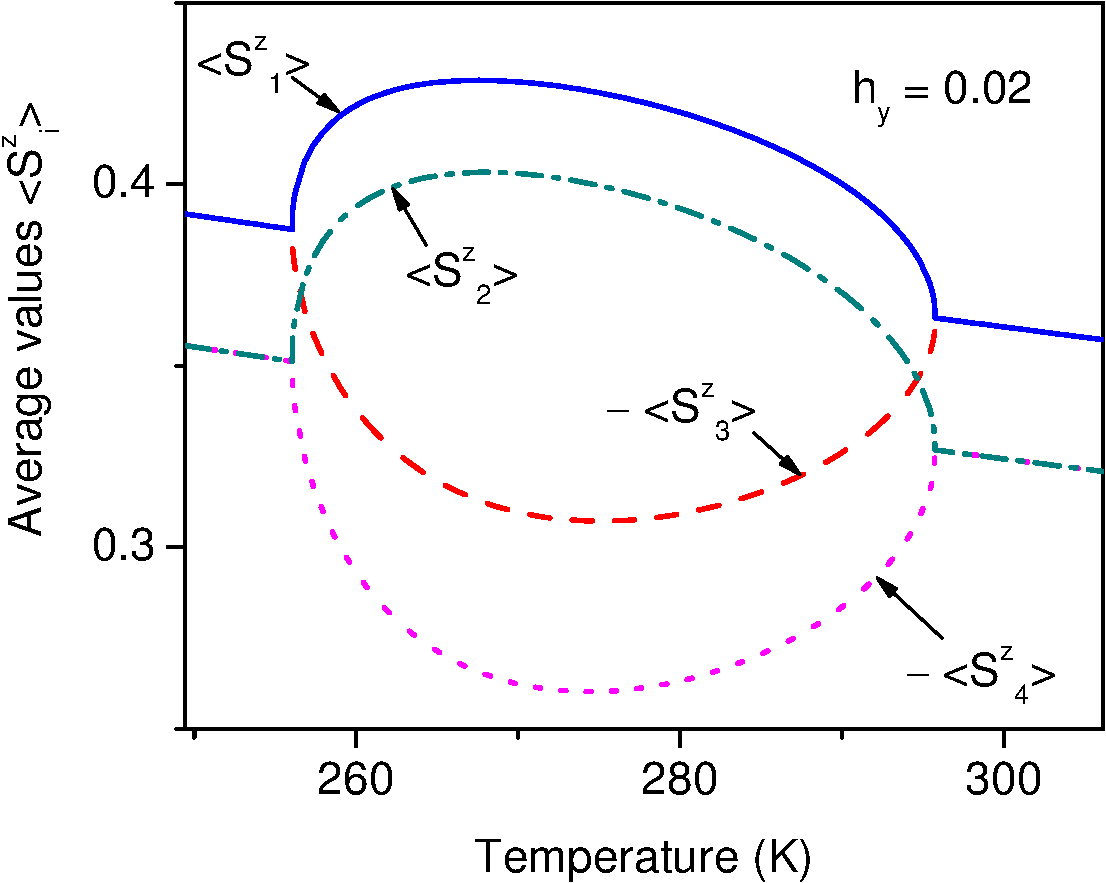
\includegraphics[width=0.65\textwidth]{eps_demo}
\end{document}
